% !TeX spellcheck = en_US

\documentclass[a4paper]{article}
\usepackage[utf8x]{inputenc}	% Use UTF8 characters
\usepackage[hyphens]{url}	% Proper url in the references section
\usepackage{relsize}		% Provide \mathlarger to get formula's to the correct size
\usepackage{hyperref}		% Clickable urls and references ("\pdfendlink ended up in different nesting level than \pdfstartlink"? add [draft])
\usepackage{enumitem}		% Numbered items, enumerate customizers
\usepackage{graphicx}		% Images
\usepackage{tabularx}		% Tables
\usepackage{needspace}		% Prevent sections starting when low on space
\usepackage{placeins}		% \FloatBarrier
\usepackage{longtable}		% Multi-page tables
\usepackage[nottoc,numbib]{tocbibind} % Add reference to the table of contents (and give it a chapter number)

\emergencystretch=10pt		% Allow more stretching whitespace to prevent overfull/underfilled lines.

% TODO: use \Needspace{5\baselineskip} before sections (redefine sections?)
\usepackage[usenames, dvipsnames]{color}
\usepackage[toc,page]{appendix}
\definecolor{inline}{rgb}{0,0,0.5}
\pagenumbering{arabic}		% Page numbering
\setlist{itemsep=0pt, topsep=2pt} % Smaller spacing between items
% \overlap for week numbers that are used twice
\definecolor{overlap}{gray}{0.5}
\newcommand{\overlap}[1]{\textcolor{overlap}{#1}}

\newcommand{\sectionbreak}{\clearpage} % Newpage before starting new section

% Setup section header spacing
\usepackage{titlesec}
\titlespacing*{\section}
	{0pt}{0.7cm}{0cm}
\titlespacing*{\subsection}
	{0pt}{0.7cm minus 0.4cm}{0cm}
\titlespacing*{\subsubsection}
	{0pt}{0.4cm minus 0.2cm}{0cm}

% Setup captions styling
\usepackage{caption}
\captionsetup[figure]{format=plain, singlelinecheck=false, margin=0pt, font={bf,footnotesize}, justification=centering, aboveskip=3pt}
\captionsetup[table]{format=plain, singlelinecheck=false, margin=0pt, font={bf,footnotesize}, justification=centering, aboveskip=3pt}
\captionsetup[lstlisting]{format=plain, singlelinecheck=false, margin=0pt, font={bf,footnotesize}, justification=centering, aboveskip=3pt}

% Setup todo note command
\marginparsep 11pt
\marginparwidth 1.4cm
\usepackage{setspace}	% \setstretch
\newcommand{\todo}[1]{{\color{BurntOrange}\sffamily\textbf{todo: #1}\par}}

\setlength{\parindent}{0em} % No indenting for new paragraphs
\setlength{\parskip}{0.5em} % Empty line between paragraphs

% Spacing of tableofcontents
\usepackage{tocloft}
\renewcommand\cftsecafterpnum{\vskip0pt}

% Code listings
%===== Code snippet styling =====
\newcommand{\code}[1]{\texttt{\small \color{inline}#1}} % \code command for inline snippets
\usepackage{listings}		% Code snippets
\usepackage{color}			% Code highlighting colors
\definecolor{dkgreen}{rgb}{0,0.6,0}
\definecolor{inline}{rgb}{0,0,0.5}
\definecolor{gray}{gray}{0.2}
\definecolor{codeText}{rgb}{0.1,0.1,0.1}
\definecolor{mauve}{rgb}{0.58,0,0.82}
\lstset{frame=tb,
	framerule=0.2pt,
	language=Java,
	aboveskip=2mm,
	belowskip=5mm,
	showstringspaces=false,
	columns=flexible,
	basicstyle={\small\ttfamily\color{codeText}},
	numbers=left,
	numbersep=4pt,
	numberstyle=\tiny\color{gray},
	keywordstyle=\color{blue},
	commentstyle=\color{dkgreen},
	stringstyle=\color{mauve},
	breaklines=true,
	breakatwhitespace=true,
	tabsize=4
}
\lstdefinelanguage{YAML}
{%
	alsoother     = @\$,
	morecomment   = **[l]{\#},
	morecomment   = **[s]{/*}{*/},
	morestring    = **[s]{"}{"},
}[keywords,strings,comments]

\lstdefinelanguage{JSON}
{%
	string       = [s]{"}{"},
	stringstyle  = \color{blue},
	comment      = [l]{:},
	commentstyle = \color{black},
}[strings,comments]

\lstset{language=C, escapechar=`} % Set default language to C
% Enable using math mode in code
\lstset{
	mathescape=true
}

\begin{document}

\begin{titlepage}
	\begin{center}
		{\huge\bfseries Verification of the Prefix Sum Program in an OpenCL Environment\par}
		
		\vspace{1cm}
		{\LARGE Thijs Wiefferink\par}
		{\large thijs@wiefferink.me, s1366564}
		
		\vfill
		
		{\Large
			University of Twente		
		}
	\end{center}

\end{titlepage}
\newpage


\section*{Abstract}
\todo{write}


\section*{Keywords}
\todo{write}


\section*{Preface}
This project is the continuation of my bachelor thesis project, in which the verification of the prefix sum algorithm has been started. Since only the 'data race free' part has been proven for the first part of the algorithm (the upsweep), the goal of this project is to prove the complete algorithm data race free, and additionally prove the functionality of the algorithm.

The necessary background information will be included in this report to understand the goal and results of the project, but full details of the Bachelor project can be read in the paper of that project \cite{bachelorThesis}.


\newpage
\tableofcontents


\section{Introduction}
This chapter describes the research domain, shows the problem that is solved, introduces the research questions and explains the approach.

\subsection{Research domain}
In this section the context information of this research project is described.

\subsubsection{GPU computing}
A graphics processing unit (GPU) is a device designed to rapidly manipulate and alter memory to accelerate the creation of images, for example while watching a video or playing a game. However, GPUs are also used more for general purpose computing, which is traditionally handled by the central processing unit (CPU). GPUs are better than CPUs doing parallel execution on large data sets. For example increasing the brightness of an image is easily done by a GPU, since this operation can be done in parallel on all pixels of the image. GPUs are however also used for physics calculations or mining crypto currencies. When using a GPU for general computing an API has to be used, I have chosen OpenCL for the previous research project because of its hardware vendor independency and open source nature. 

Running a parallel computation on a GPU brings a couple of challenges. The first challenge is preventing data races. A data race is the situation in a program where multiple threads are accessing the same memory location, with at least one of them writing to the location. The second challenge is verifying the correctness of the functionality of the program. Verifying both of these aspects is useful for safety critical systems.

The previous research project has started with the verification process to show that a program (specifically the Prefix Sum algorithm) has no data races. Since only the first half of the program could be verified in the given time for the project the verification has been continued in this project.

\subsubsection{Prefix Sum}
To show what the prefix sum is and how it is calculated, this section repeats the information from the previous project\cite{bachelorThesis} below.

The algorithm computes the sums of all possible prefixes of an input array. In Figure~\ref{prefixsumexample}, a mathematical representation of the prefix sum is illustrated, $x$ represents the input array, $x_0$ indicates the first element from the input array, where $n$ represents the size of the input array, and $y$ is the output array containing the prefix sums. Each number $y_a$ in the output array is the sum of all numbers $x_b \in x$ for which the condition $b<a$ holds.

\begin{figure}[htb!]
	\centering
	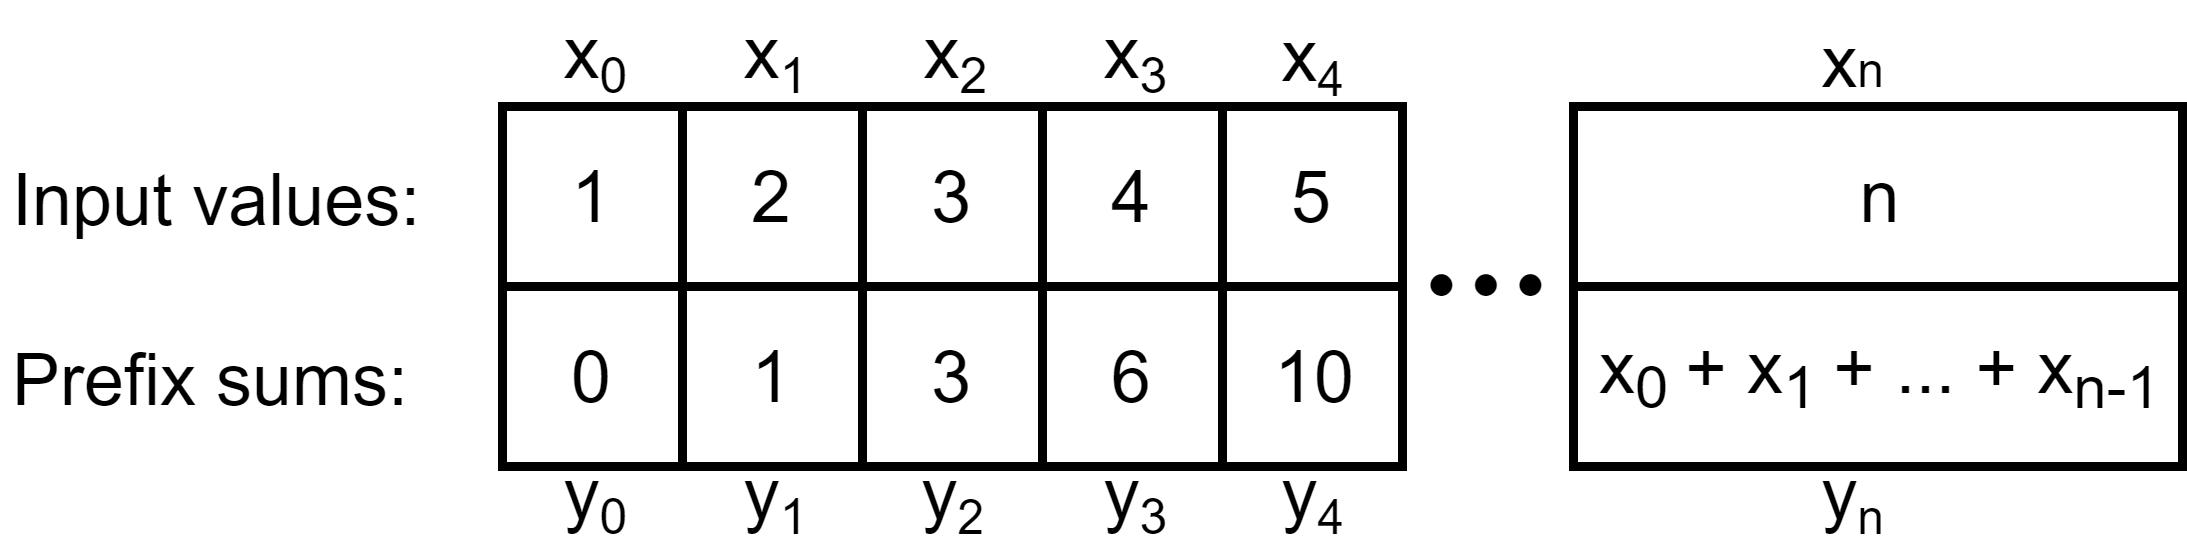
\includegraphics[width=80mm]{../images/prefix-sum-v1.png}
	\caption{Prefix Sum description}
	\label{prefixsumexample}
\end{figure}

The Prefix Sum algorithm is an interesting case study because it is a building block for a lot of other algorithms. For example radix sort and quicksort can be implemented using Prefix Sums, but it can also be used to lexically compare strings of characters or to search for regular expressions \cite{Blelloch:PrefixSumApplications}. In the field of specifying and verifying GPU programs the Prefix Sum is a suitable next step, because it will be a bigger and more complex example of verifying a GPU program.

The algorithm to calculate prefix sums can be structured in such a way that large amounts of data can be processed in parallel. A multi threaded algorithm meant for the GPU has been implemented in the previous project. The verification process continues with this same algorithm. The implemented version of the Prefix Sum is based on Chapter 39 \emph{Parallel Prefix Sum (Scan) with CUDA} of the book GPU Gems 3 \cite{Nguyen:GPUGems3}.

\subsubsection{Verification}
For the verification of the Prefix Sum program Permission-Based Separation Logic is used to specify the behavior of the program, and the tool VerCors is used to verify that the code matches the specification. A description of Permission-Based Separation Logic can be found in the previous project\cite{bachelorThesis}. 

\subsection{Problem statement}
Making sure a program has no data races, and always gives correct results is extremely hard, if not impossible with traditional testing. For a single-threaded application testing all inputs should prove that the program is correct, but for multi-threaded applications this does not prove anything about data races. In order to verify the correctness of a program it has to be specified in Permission-Based Separation Logic, which is a challenge for bigger programs like the Prefix Sum. VerCors, the tool used to verify the specification, will get slower when a larger specification is used. This makes using the tool correctly and efficiently a challenge. During the previous project a number of problems in the tools have been identified that blocked the verification, during this project this will be the case as well.

\subsection{Research questions}
The following research questions have been formed from the problem statement:
\begin{enumerate}
	\item How can the Prefix Sum program be proven to have no data races?
	\item How can the Prefix Sum program be proven to give the correct result?
	\item What are the limitations of VerCors for verifying GPU programs?
\end{enumerate}

The first research question has partially been proven by the previous research, which will be used as a starting point. To answer it fully the specification of the Prefix Sum algorithm has to be extended to the complete program (add the downsweep and final permissions). For the second research question the specification created for the first question has to be extended with information about the results. The third question is to review the VerCors tool, which will be done during the verification process of the first two questions.

\subsection{Approach}
First the last specification of the previous project will be tested in the last version of VerCors, to ensure it still works after all changes in tool. After that works, the verification of the read/write permissions can be continued for the downsweep phase of the program. I expect that the specification should not be hard, because it uses much of the same patterns of the upsweep phase, but getting VerCors to actually verify it will take time. After the downsweep phase is specified and verified, the \code{ensures} clause of the complete program can be added, which might give some trouble to proof as well. While adding more specifications I expect the verification time to increase. Hopefully this does rise to a time that makes iterating through different versions of the specification too slow.

After the read/write permissions have been verified, the functional specification and verification can be started. To speed up this process it is probably best to remove the downsweep phase at first, and just start with the upsweep phase. This will keep the iteration time low and should make it easy to rapidly expand the specification. Doing the verification of the downsweep phase might get slow due to the verification time of VerCors. Adding the final ensures for the complete program might be the hardest task, since the everything needs to be enabled at that point.

To answer the third research question notes will be made during the verification process to keep track of tool improvements and limitations. These will be written down to provide future work for the tool, or notes for creating specifications that are supported by VerCors.

When encountering a problem during the verification, Stefan Blom (author of VerCors) will be contacted to see if there is a problem in VerCors and if/how that could be solved.

\subsection{Report structure}
\todo{introduce chapters}


\section{Prefix sum algorithm}
The sections below are repeated from the previous project\cite{bachelorThesis}, describing the algorithm that is used for calculating the Prefix Sum in parallel.

\subsection{Prefix Sum algorithm} \label{implementBasic}
The basic single thread Prefix Sum algorithm is simple, but cannot be used with multiple threads. The trivial way to compute Prefix Sums would be to compute it as described in Listing~\ref{singleThreadAlgorithm}. In the loop body of this algorithm it depends on knowing the result of the previous sum, because of this data dependency the algorithm cannot be used to calculate Prefix Sums concurrently. 

\begin{lstlisting}[caption=Single thread Prefix Sum, label=singleThreadAlgorithm, float=htpb]
result[0] := 0
for a := 1 to n do  
	result[a] := input[a-1] + result[a-1]
\end{lstlisting}

The algorithm implemented for this research is made by Blelloch \cite{Blelloch:PrefixSum}, and can be used concurrently. The description of Nguyen \cite{Nguyen:GPUGems3} has been followed to implement the algorithm. The \emph{Simple-OpenCL} library \cite{Huguet:SimpleCL} of O. A. Huguet and C. G. Marin has been used to implement the OpenCL kernels. The algorithm by Blelloch performs the Prefix Sum calculation in two phases, the up-sweep phase and down-sweep phase. The algorithm uses a balanced binary tree for data storage, therefore a tree with $log_2(n)$+1 levels is required to accommodate for an input of size \emph{n}. If the input size is not a power of 2, then the input will be padded with zeros until it is; this is necessary because the algorithm requires a binary tree. The tree has $d=log_2(n)$+1 levels, and each level $d$ has $2^d$ nodes. At the start the input values will be placed in the \emph{n} leaves at the bottom of the tree, see Figure~\ref{treeStart}. The up-sweep phase traverses the tree from the leaves to the root, level by level, and computes partial sums in the nodes of the tree. At each level the sum of 2 nodes is computed and placed in the node above, at the end the root node contains the sum of all elements in the input. Figure~\ref{treeUpSweep} shows the end result of this phase.

\begin{figure}[htb!]
	\centering
	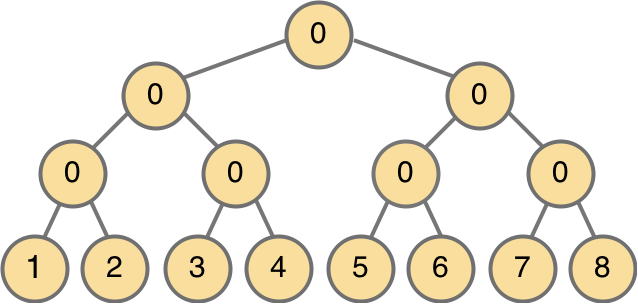
\includegraphics[width=80mm]{../images/tree-start.png}
	\caption{Tree at the start of the up-sweep phase}
	\label{treeStart}
\end{figure}

\begin{figure}[htb!]
	\centering
	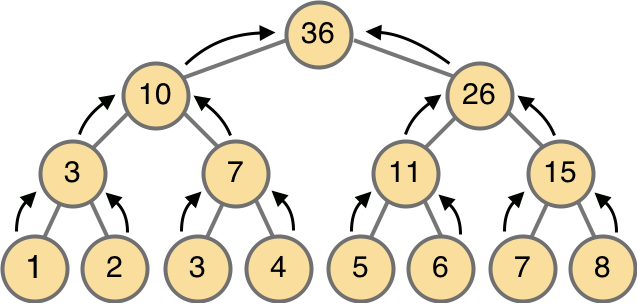
\includegraphics[width=80mm]{../images/tree-upsweep.png}
	\caption{Tree after the up-sweep phase}
	\label{treeUpSweep}
\end{figure}

After this first phase the second phase will start, called the down-sweep phase. This phase starts by inserting zero at the root of the tree, after that it traverses the tree from the root to the leaves. On each level the right child will be set to the sum of the left child and the current node, and the left child will be set to the value of the current node. This way the zero that has been inserted at the root will travel to the leftmost leaf, and intermediate sums will travel to the right, and get added to form the final result. Figure~\ref{treeDownSweepFirst} illustrates the first step, the right node will get the value $0+10$, the left node will get value $0$. Figure~\ref{treeDownSweepSecond} shows the result of the second step, and Figure~\ref{treeDownSweepFinal} shows the end result, with an exclusive prefix sum in the leaves of the tree. An exclusive prefix sum means that each output value is the sum of all inputs with a lower index, instead of a lower or the same index as with an inclusive prefix sum.

\begin{figure}[htb!]
	\centering
	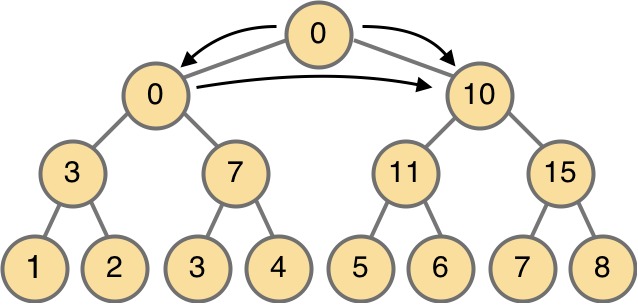
\includegraphics[width=80mm]{../images/tree-downsweep-first.png}
	\caption{The first step of the down-sweep phase}
	\label{treeDownSweepFirst}
\end{figure}

\begin{figure}[htb!]
	\centering
	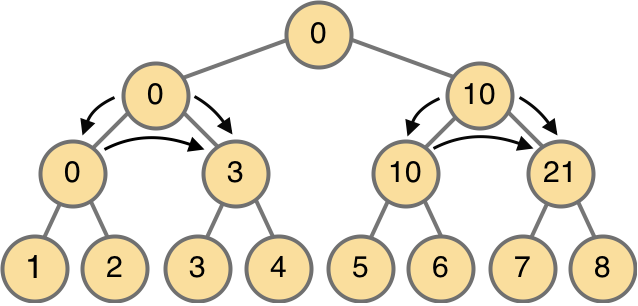
\includegraphics[width=80mm]{../images/tree-downsweep-second.png}
	\caption{The second step of the down-sweep phase}
	\label{treeDownSweepSecond}
\end{figure}

\begin{figure}[htb!]
	\centering
	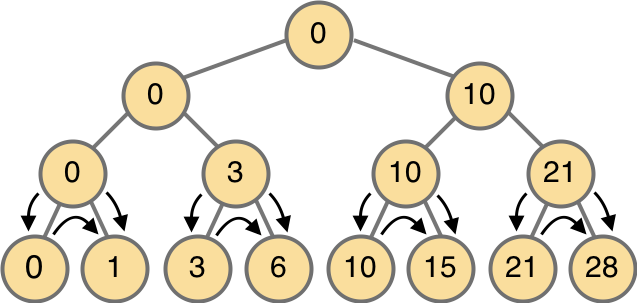
\includegraphics[width=80mm]{../images/tree-downsweep-final.png}
	\caption{The final step of the down-sweep phase}
	\label{treeDownSweepFinal}
\end{figure}
\FloatBarrier

\subsection{Two-dimensional Arrays As Storage} \label{prefixSumStorage}
Now that the algorithm of the Prefix Sum has been explained in Section~\ref{implementBasic}, the storage of the tree in memory will be looked at. A common way to store a binary tree in an array is to have the root node at index $i=1$, with the left child at $i*2$ and the right child at $i*2+1$. Such a storage solution would require an array of twice the size of the input, which is the minimum required size for this algorithm to work. The disadvantage of this storage type is that at each level of the tree in the up- and down-sweep phase only a part of the threads running the kernel are active. To illustrate, in the example of Figure~\ref{treeUpSweep} about the up-sweep phase, 4 threads would be required to run this kernel, with 4 of them active on the lowest level, then 2 on the level above, and 1 for the highest level. To make the correct threads active and idle, the kernel has code that shuts off certain threads in certain iterations of the up-sweep phase. This code causes branch divergence, which means that certain threads of a kernel are running different code as other threads. Because threads run different code, the SIMT principle is disturbed.

To prevent the problem mentioned above a different version of the Prefix Sum algorithm has been implemented that uses another storage solution for the binary tree. The algorithm has a two-dimensional array, the first array stores an array for each level of the tree, and those levels have values for each node of the tree. The two-dimensional array has a height of $log_2(n)$+1, and a width the same as the inputsize n. The nodes of a tree are aligned to the left in the level arrays, which leaves blank spots on all levels except the lowest one. Because of these blank spots we can now let all threads do the calculation as explained in Section~\ref{implementBasic}. The threads that normally would have been idle will now perform operations on the blank spots of the two-dimensional array, which do not interfere with the actually useful calculations. This change has a positive effect on the performance of the kernel because of reduced branch divergence \cite{Han:ReducingBranchDivergence}. The kernel of the one-dimensional array would need to be split each time it is executed, since there are threads executing different code. But this is not the case for the two-dimensional array version, in which all threads do exactly the same operations (although on different data). The previous research project has benchmarked the two solutions and confirmed that the two-dimensional array has better performance.

\subsection{Algorithmic description} \label{sec:implAlgorithmic}
The algorithm with the two-dimensional arrays works as described in Listing~\ref{prefixSumUpsweep} (up-sweep phase) and Listing~\ref{prefixSumDownsweep} (down-sweep phase). The loops at respectively line 2 and line 3 of these algorithms are to indicate that one work item of the GPU will do the calculation inside the loop. The arrays used in the algorithms have their first dimension represent the level of the tree, and their second dimension the node of tree on the given level. The algorithms assume that the values of the nodes of the tree are stored as much to the left as possible, so for example the root of the tree has 0 as the second dimension of the array, and the highest possible number on the first dimension: $log_2(n)-1$.

\begin{lstlisting}[caption=Upsweep phase, label=prefixSumUpsweep, float=htpb]
for d=1 to `$log_2(n)$` do
	for all k=0 to n-1 in parallel do 
		x[d][k] := x[d-1][k*2] + x[d-1][k*2+1]
\end{lstlisting}

\begin{lstlisting}[caption=Downsweep phase, label=prefixSumDownsweep, float=htpb]
x[(`$log_2$`(n)-1)*n] := 0
for d=`$log_2$`(n)-1 to 1 do
	for all k=0 to n-1 in parallel do
		x[d-1][k*2+1] = x[d-1][k*2] + x[d][k]
		x[d-1][k*2] = x[d][k]
\end{lstlisting}
\FloatBarrier


\section{Verifying permissions}
This chapter describes the process of verifying the read/write permissions of the Prefix Sum program. It starts with the result of the previous research, expands it to the downsweep phase, after which the specification is simplified.

\subsection{Starting point}
Listing \ref{specification:previous} shows the specification as was made during the previous project. This specification has been verified until the end of the upsweep phase. The specification of the downsweep phase has been written down, as well as the ensures for the complete program, but these could not be verified by VerCors yet at that time.

This specification is a good starting point for completing the read/write permissions verification. The process of extending this specification is described in the next section.

\lstinputlisting[
	caption={
		Specification as written in the previous project,\\
		only the upsweep part is verified
	},
	label=specification:previous,
	linewidth=13cm,
	basicstyle={\scriptsize\ttfamily\color{codeText}}
]{specifications/previous.pvl}

\subsection{Verifying downsweep array permissions}
Listing \ref{specification:basic} shows the working specification of all permissions of the \code{input}, \code{output} and \code{temp} array. The specification made in the previous project was quite close, but required some adjustments to verify with VerCors. First the permissions that should be active are explained, after which the required specification updates are shown.

\subsubsection{Input array permissions}
The input array permissions are shown in Figure \ref{fig:inputArrayPermissions}, the array indices are shown at the bottom, the numbers inside the squares indicate the thread number that has access. The figure shows the input array for an input size of 8. This means that there will be 8 thread, of which only the first 4 will get any permissions. Each thread has access to indexes $t*2$ and $t*2+1$, where $t$ is the thread number. In the upsweep phase the first half of the threads will start adding inputs together in consecutive pairs, so that is why the input array permissions are distributed like this.

\begin{figure}[htb!]
	\centering
	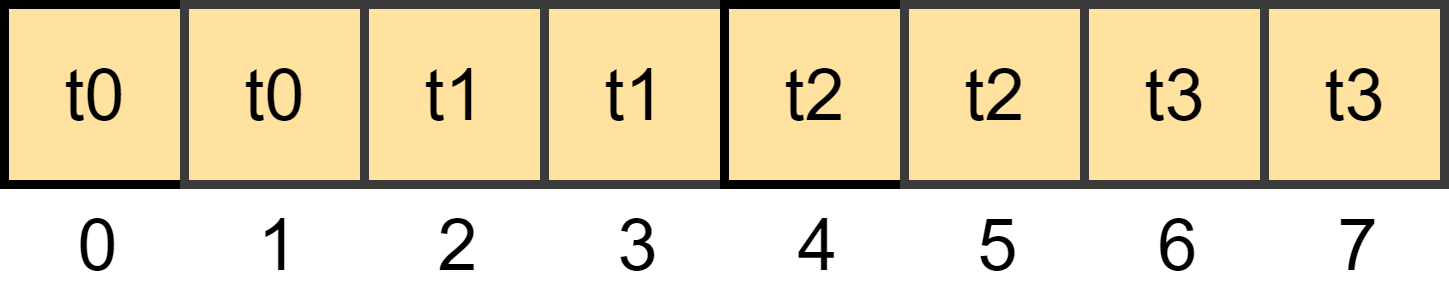
\includegraphics[width=80mm]{../images/input-permissions-v1.png}
	\caption{Permissions of the input array}
	\label{fig:inputArrayPermissions}
\end{figure}
\FloatBarrier

\subsubsection{Tree array permissions}
The tree array permissions are more complex, and will change during the up and downsweep. At the start of the program the permissions are as shown in Figure \ref{fig:treeArrayPermissionsStart}. This figure shows the tree array with $N$ horizontally and $H$ vertically. The numbers in the squares show which thread has write access. A part of the squares have no background color, these are still included, but serve no actual purpose other than improving performance by reducing branch divergence as shown in the previous research project.

The permissions of the bottom row ($H=0$) are like the input array, each thread has access to index $t*2$ and $t*2+1$. In the other rows the indices are simply assigned to their thread number. The first step of the downsweep will start with $tree[1][0] = tree[0][0] + tree[0][1]$, which thread 0 can do because it has write permissions to each of these locations. Thread 1, 2 and 3 have permissions to the next locations, doing the same computation as thread 0 while adjusting their indices using the thread number.

With the initial permissions of the input array and the bottom row of the tree array, the input can be copied to the bottom row of the tree array. The first half of the threads will do this task, each copying two consecutive locations, again $t*2$ and $t*2+1$.

\begin{figure}[htb!]
	\centering
	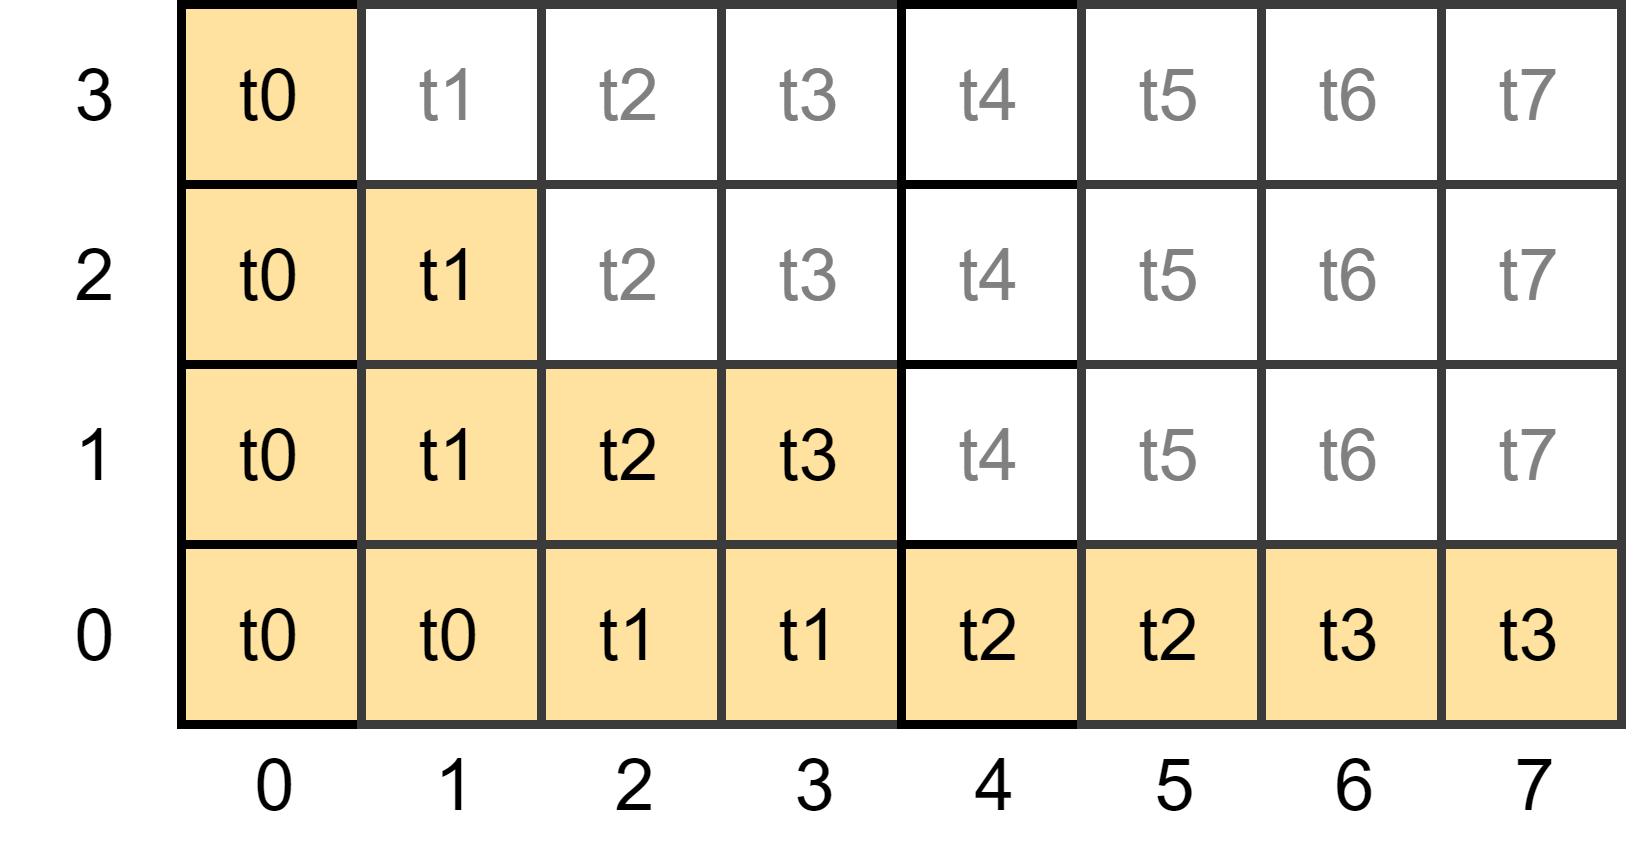
\includegraphics[width=80mm]{../images/tree-permissions-start-v1.png}
	\caption{Permissions of the tree array before starting the upsweep}
	\label{fig:treeArrayPermissionsStart}
\end{figure}
\FloatBarrier

The \code{barrier()} of the upsweep will update the tree permissions row-by-row. Each iteration of the while loop the permission layout of the bottom row is applied to the next row above, until all but the top-most row has that permission layout. The resulting permissions are shown in Figure \ref{fig:treeArrayPermissionsMiddle}.

\begin{figure}[htb!]
	\centering
	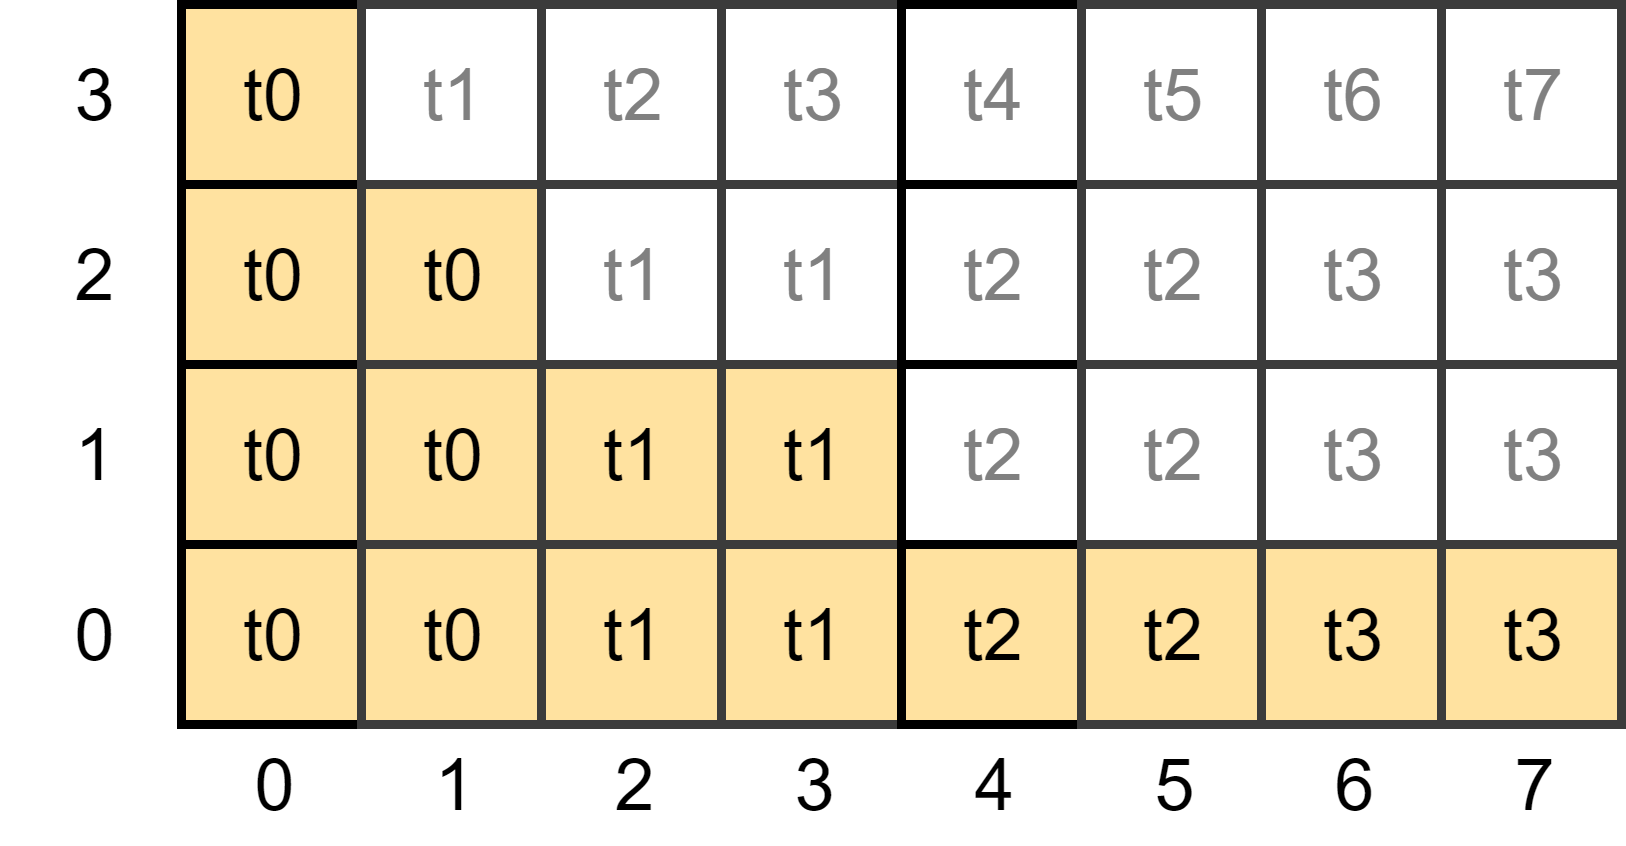
\includegraphics[width=80mm]{../images/tree-permissions-middle-v1.png}
	\caption{Permissions of the tree after upsweep}
	\label{fig:treeArrayPermissionsMiddle}
\end{figure}
\FloatBarrier

After the upsweep the program will set the root of the tree to zero, each thread has still access to the cell of its thread id, so each thread updates one cell.

Now the downsweep can start, for which the starting permissions are as shown in Figure \ref{fig:treeArrayPermissionsMiddle}. For all rows below the top-most row, the first half of threads will update two cells, at $t*2$ and $t*2+1$. The first computation can immediately start, because the permissions are already correct. For the following rows the permissions need to be updated row-by-row, reverting the permissions that have been added for the upsweep. After the downsweep the permissions will look as shown in Figure \ref{fig:treeArrayPermissionsEnd}.

\begin{figure}[htb!]
	\centering
	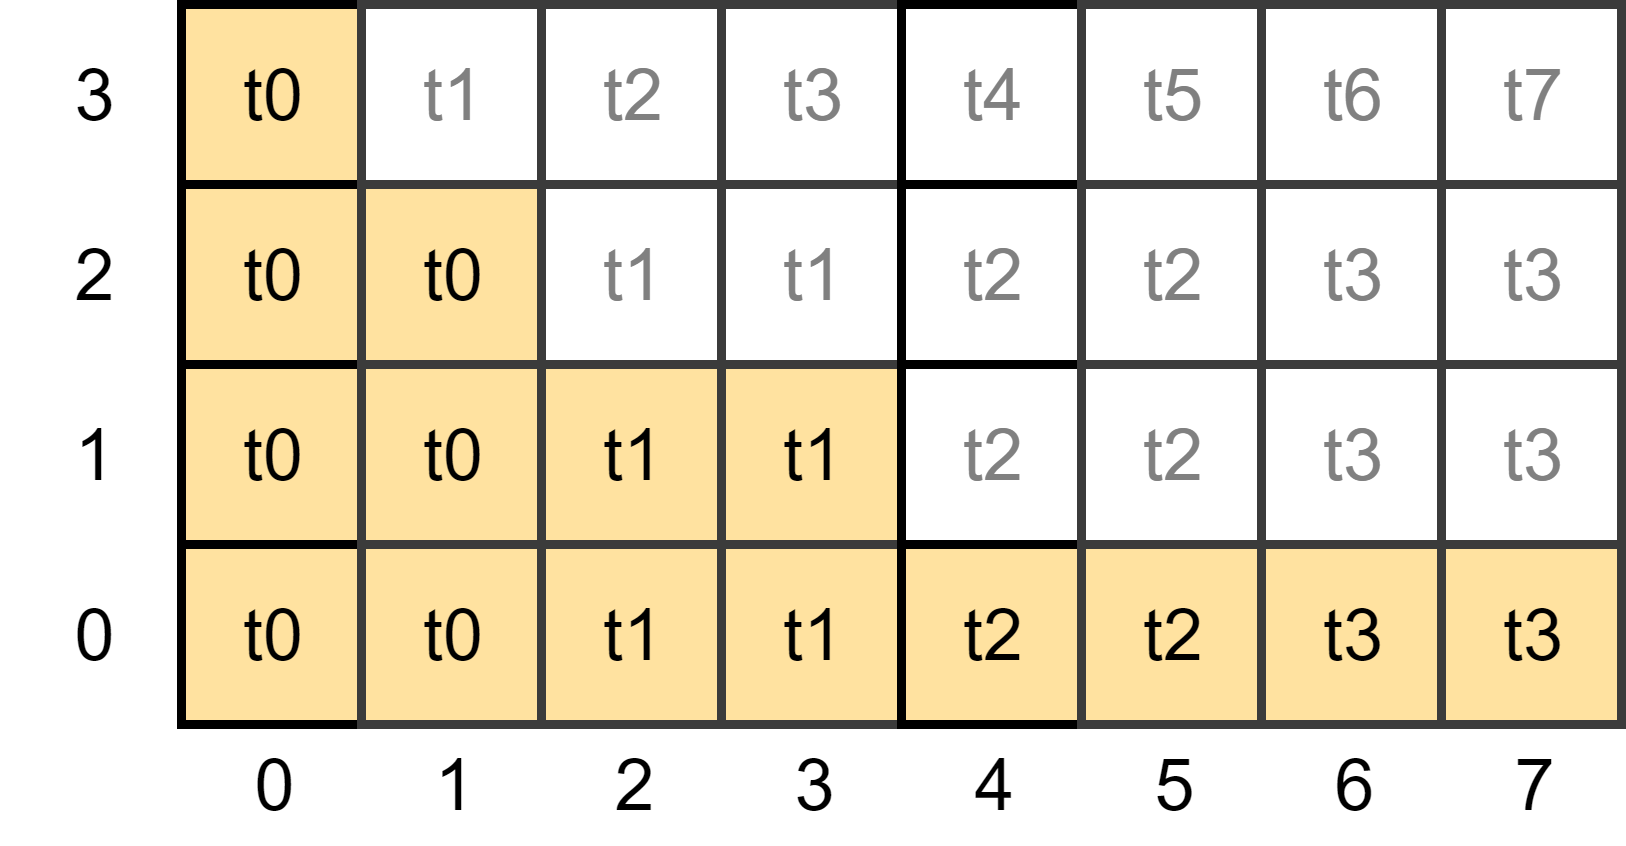
\includegraphics[width=80mm]{../images/tree-permissions-middle-v1.png}
	\caption{Permissions of the tree after the downsweep}
	\label{fig:treeArrayPermissionsEnd}
\end{figure}
\FloatBarrier

\subsubsection{Output array permissions}
At the end of the computation the result is at the bottom row of the tree array and will be copied to the output array. The bottom row of the tree array still has the layout where each thread has access to $t*2$ and $t*2+1$. So to easily copy the results the output array should have the same permission layout. The resulting permission layout is the same as the input array as shown in Figure \ref{fig:inputArrayPermissions}. Now the first half of threads can copy the result and the Prefix Sum computation is complete.


\subsubsection{Specification changes}
Below the changes to the specification of the previous research project are explained.

\textbf{Merged barrier clauses}\\
The barrier of the upsweep phase changes the permissions, as described above in the permissions layout. The original specification used one require, and two ensures in the barrier to accomplish this change, as shown in Listing \ref{listing:specPreviousBarrier}. VerCors could not match these statements correctly through the while loop, to solve this problem the ensures clauses have been merged into one ensure clause, as shown in Listing \ref{listing:specBasicBarrier}. Both of these options mean exactly the same, but is is hard for VerCors to recognize the original one. Ideally this would be fixed in the tool, but this was not trivial. This alternative notation has been provided by the tool author.

\begin{lstlisting}[caption=Upsweep barrier permissions clauses (before merging), label=listing:specPreviousBarrier, float=htpb]
requires Perm(tree[level-1][t], write));
ensures t<(N/2) ==> Perm(tree[level-1][t*2], write));
ensures t<(N/2) ==> Perm(tree[level-1][t*2+1], write));
\end{lstlisting}

\begin{lstlisting}[caption=Upsweep barrier permissions clauses (after merging), label=listing:specBasicBarrier, float=htpb]
requires Perm(tree[level-1][t], write));
ensures t<(N/2) ==> (\forall* int k; 0<=k && k<2; Perm(tree[level-1][t*2+k], write));
\end{lstlisting}

A similar merge was required for the downsweep barrier, in this case two require clauses have been merged into a single one using the same technique.

\textbf{First step of the downsweep}\\
The first iteration of the downsweep has been extracted from the while loop. This was necessary because the permission layout of the tree array was already correct for the first iteration, so doing a barrier was not necessary yet. Extracting this first iteration leads to code duplication for the downsweep operation, which will be addressed in later specification versions. This change also meant updating the loop\_invariant of the downsweep while loop, the \code{level<i} has been replaced with \code{level<=i} in the loop\_invariant that describes the write permissions of the temp array of all rows except the bottom one.

\textbf{Array definition workaround}\\
VerCors did not properly recognize the length of the array through the specification, and could sometimes not know that each specified array cell is unique. A workaround for this problem has been provided by Stefan Blom. By adding \code{tree != null} the tools handles array lengths correctly and knows its cells are unique. Hopefully this workaround can be removed in the future.

\textbf{Assert statements}\\
The VerCors tools could not get through the while loops correctly anymore after some updates, the underlying problem is in the external library Z3. This problem has been solved by adding \code{assert <condition>} statements just before and inside the barrier, and by using identity operators in some places. These statements force the tools to prove a certain condition at that point, which provides provides search options into the right direction (where previously the tools would run out of options). At the end the specification works, but got bigger with assert statements and has added complexity with identity operators \code{id(0)} and \code{id(1)}.

\textbf{Simplification failures}\\
A couple of "simplification failure" errors have been encountered during the verification process. This happens when a \code{\\forall*} cannot be transformed to a rule that the internal prover accepts. Transformations like these happen with simple matching rules, that replace certain parts with others. For example a simplification failed at some point when instead of writing \code{0<=i \&\& i<N}, I wrote \code{i>=0 \&\& i<N}. These expressions mean the same exact thing, but the rules only match the first variant. These kind of problems would really need to be solved before VerCors can be used by anyone to verify their programs.

\textbf{Cleanup}\\
Inside the barrier of the upsweep there was an unnecessary ensures clause, which has been removed: \code{ensures Perm(tree[level][t], write));}.
Additionally the ensures clause of the complete program has been simplified, it does not have a separate clause for the bottom row of the tree array anymore. The split clauses were not necessary, since the program simply has write permissions to all locations in the tree array, so it is pointless to split among multiple clauses.

\textbf{Verification time}\\
A side effect of all changes is that the time it takes to verify the specification went from around 2 minutes, to 6 minutes. Considering that the Prefix Sum is quite a trivial number of lines of code, this is quite long. This would prevent verifying large programs, because it simply takes too long to run, especially considering that the specification is rarely correct the first run. The author of the tool indicates that each \code{if} statement causes the verification time to go up, since there are more options to consider. Loops have an even larger impact, which is why this program saw the increase in verification time. The workaround with \code{assert} and \code{id()} also do not help performance.

\subsubsection{Result}
After the changes described above the specification is complete and verifies in VerCors. It proves that the program does not contain data races, which is a good step towards proving the complete program.

\lstinputlisting[
	caption={
		Full permissions specification, verified using VerCors
	},
	label=specification:basic,
	linewidth=13cm,
	basicstyle={\scriptsize\ttfamily\color{codeText}}
]{specifications/basic.pvl}

\subsection{Specification simplification}
After finishing the specification for the array permissions, it felt like it was too verbose. The first problem is that a lot of clauses start with \code{t<(N/2)}, and most code blocks are also have the same condition. This condition disables the last half of the threads that are used in the kernel. Actually these threads are not useful at all and normally would not be used for the execution. The only reason the number of threads is double than necessary is that VerCors could not handle the correct number of threads at first. The syntax of specifying a GPU kernel program was different, and did not allow to easily use half the number of threads, and arrays did not accept expressions inside their declaration. Later the syntax updated based on the Java language syntax, so it basically is just a class with a method inside. So now it is possible to make a specification with half the number of threads, so that the result is a lot more compact and readable. The resulting specification will be discussed below.

\subsubsection{Half the number of threads}
To half the number of threads the \code{N==32} clause has been changed to \code{N==16}. The \code{par} block that specifies the number of threads uses the N directly, so the number of threads is now correctly halved. The input, output and tree array specifications are changed to use $N*2$ as size, because they should stay the same size as before.

\subsubsection{Compacting: invariant and context keywords}
In the previous specification the clause \code{N==32 \&\& H==6} was repeated constantly, in each loop and barrier. To prevent this kind of repetition the \code{invariant} keyword is now available on the program level, so that specifying constants is only needed once. This cleans up a lot of clauses, making the specification easier to read and understand.

Another pattern that is common in the previous specification is that a clause in the requires and ensures is the same. For example the barrier would repeat a condition of the loop\_invariant as a require and ensure, duplicating this specification. This has been solved by Stefan Blom by adding the \code{context} keyword in VerCors, which acts as a require and ensure at the same time. This compacted the specification of the barriers a bit, for the constraints of the thread number and the level.



\subsubsection{Updated permissions loop\_invariants}


\subsubsection{Merged first iteration}


\lstinputlisting[
caption={Compacted specification using only half the number of threads},
label=specification:halfthreads,
linewidth=13cm,
basicstyle={\scriptsize\ttfamily\color{codeText}}
]{specifications/halfthreads.pvl}

\todo{Write about:}
\begin{enumerate}
	\item context clauses
	\item N==16
	\item New loop\_invariants of the while loops
	\item Folded first iteration into the while loop, swapped computation and barrier in downsweep
	\item Discussions with Stefan
	\item \textbackslash matrix and \textbackslash array (removed tree!=null)
\end{enumerate}


\vspace{3cm}
\todo{Steps:}
\begin{enumerate}
	\item Show version of previous research
	\item Extend to downsweep and program ensures (Permissions V2, show the encountered problems)
	\item Half threads version (HalfThreads, show encountered problems)
	\item Explain functional ideas (new permissions layouts)
\end{enumerate}


\section{Verifying functionality}
\todo{verification process of the functionality of the program}


\section{Discussion}
\todo{summary}

\subsection{Verification performance}
\todo{Current performance, options and solutions for the future}
\begin{enumerate}
	\item Scaling with classes
	\item Scaling with methods
	\item Improvements in Z3
	\item Better hardware
	\item Better progress during verification
\end{enumerate}

\subsection{Results}

\todo{result description: verified}

\subsection{Related work}
\todo{similar verification projects}


\section{Conclusion}
\todo{summary}

\subsection{Research question answer}
\todo{works, not for huge programs though}

\subsection{Limitations and problems}
\todo{tool limitations, change code for verification process}

\subsection{Research value}
\todo{do larger programs, improve tool, concurrency}

\subsection{Future work}
\begin{enumerate}
	\item Larger programs
	\item Improve tool
	\item Handle more functional details: overflow, underflow, etc.
\end{enumerate}

\bibliographystyle{abbrv}
\bibliography{Report}

\end{document}
